\documentclass{article}
\usepackage[utf8]{inputenc}
\usepackage{indentfirst}
\usepackage{listings}

\title{Oscar Search}
\author{fanfaredash, 2019201407}
\date{July 2020}

\usepackage{natbib}
\usepackage{graphicx}

\begin{document}

\maketitle

\section{Introduction}

This project is a simple \emph{offline web-search program} implemented with web-crawler technology, inverted index, and TF-IDF.

With this project, you can first get all web-pages under the root URL, which is specified, then use search-engine module to query web-pages.

\section{Usage}

\begin{itemize}
    \item Requirements
    \item Installation
    \item Initialization
    \item Searching
    \item Settings
\end{itemize}

\subsection{Requirements}
Python3 (\geq 3.5.2)
\\

\subsection{Installation}
Run following code in \emph{bash} to install basic packages:\\

\begin{tabular}{|l|}\hline\begin{minipage}[t][1em]{20em}\begin{verbatim}
sudo pip3 install -r requirements.txt
\end{verbatim}\end{minipage}\\\hline\end{tabular}
\\

\subsection{Initialization}
That is, to download and prepare data for search-engine.

First, go to \emph{arguments.py}, and change argument \emph{root} to your target website.

For example, \texttt{root = "http://info.ruc.edu.cn/"}.

Then start \emph{run.sh}:\\

\begin{tabular}{|l|}\hline\begin{minipage}[t][1em]{4.5em}\begin{verbatim}
./run.sh
\end{verbatim}\end{minipage}\\\hline\end{tabular}\\

Or you can use \begin{tabular}{|l|}\hline\begin{minipage}[t][1em]{9.5em}\begin{verbatim}
python3 [filename]
\end{verbatim}\end{minipage}\\\hline\end{tabular} to initialize data step by step:\\

\begin{tabular}{c|c}
     
crawler\_mt.py     & getting html data from website\\
parser.py         & parsing html data for pure text\\
cutter.py         & split documents for terms\\
index.py          & building inverted index
\end{tabular}
\\

\subsection{Searching}
Start search using: \begin{tabular}{|l|}\hline\begin{minipage}[t][1em]{16em}\begin{verbatim}
python3 search.py [query_text]
\end{verbatim}\end{minipage}\\\hline\end{tabular}.

This will display result in console.\\

Or use Flask to deploy user interface: \begin{tabular}{|l|}\hline\begin{minipage}[t][1em]{5em}\begin{verbatim}
flask run
\end{verbatim}\end{minipage}\\\hline\end{tabular}

After that, use browser to access your web server.

\begin{figure}[h!]
\centering
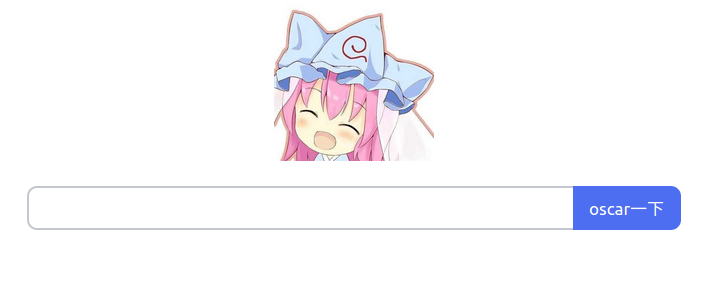
\includegraphics[scale=0.5]{1.png}
\caption{Oscar search: main page}
\label{fig:1}
\end{figure}

\newpage

\begin{figure}[h!]
\centering

\includegraphics[scale=0.5]{2.png}
\caption{Oscar search: sample}
\label{fig:2}
\end{figure}

\subsection{Settings}
Customize arguments in *arguments.py*.

\begin{tabular}{c|c}
root              & web-crawler target \\
resultDisplay     & maximum results on display \\
abstractDisplay   & maximum length of abstract (UI only) \\
\[directory arguments\] & modify file path(not recommended)
\end{tabular}\\
\\

Default file path:\\

\begin{tabular}{c|c}
html file           & /raw/html \\
page text           & /raw/text \\
page title          & /raw/title
\end{tabular}\\

\ \\

File-names are encrypted by base64 method. 

Use \begin{tabular}{|l|}\hline\begin{minipage}[t][1em]{17em}\begin{verbatim}python3 ess.py -d [filename.html] \end{verbatim}\end{minipage}\\\hline\end{tabular} to decrypt for web-page URL. 

Or use \begin{tabular}{|l|}\hline\begin{minipage}[t][1em]{16.5em}\begin{verbatim}python3 ess.py -e [web-page URL] \end{verbatim}\end{minipage}\\\hline\end{tabular} to encrypt for filename.\\

Customize stop word list in \emph{stopwords.txt}, word per line.

Customize user dictionary in \emph{userdict.txt}, word per line.
\newpage

\section{Features}

\begin{itemize}
    \item Flexibility
    \item Base64 encryption
    \item Offline index building
    \item Process-Oriented Programming
    \item Multi-Thread crawling
\end{itemize}

\subsection{Flexibility}
Compared to other projects in SPP2020 homework, this project includes \emph{no} algorithm or method related to "https://info.ruc.edu.cn/". The whole project works well with other root URLs.

Besides root URL, user can also customize number of search results and length of abstract displayed, though it's much more trivial than the former one.

\subsection{Base64 encryption}
As we know, there should be no character "/" in filename.

This project uses base64 encryption to resolve URL string. Base64 builds a bijective function between URL string and filename, which is much safer than to replace "/" to other substrings.

\subsection{Offline index building}
This project uses offline index building, which means the program won't have to build inverted index every time when the user search for result.

Offline index building also requires saving data to files, that might rise the time complexity of the program. Therefore, \emph{BKDR-hash} algorithm and \emph{binary-search} algorithm are used in term searching.

Yet due to the data scale of "https://info.ruc.edu.cn/" is only about 7000 (web-pages), this program didn't show its speed advantage in automatic test.

\subsection{Process-Oriented Programming}
The source code of this project are well process-oriented. Developers who are interested in this project can easily customize their own process and replace its counterpart in the source code.

\subsection{Multi-Thread Crawling}
This project uses multi-thread technique to speed up web-crawling process.
\end{subsection}

\end{document}